\section{Ôn tập chương 4}
\subsection{Đề 1}
\Opensolutionfile{ans}[ans/ans-2-OTC4-De1]
\caulc
\begin{ex}%[2D4N1-1]%Biên soạn:Phùng Hoàng Em %Phản biện:Nguyễn Đắc Kiên
	Hàm số $F(x)$ là một nguyên hàm của hàm số $f(x)$ trên khoảng $K$ nếu
	\choice
	{$F'(x)=-f(x),\,\forall x \in K$}
	{\True $F'(x)=f(x),\,\forall x \in K$}
	{$f'(x)=F(x),\,\forall x \in K$}
	{$f'(x)=-F(x),\,\forall x \in K$}
	\loigiai{
			Theo định nghĩa thì hàm số $F(x)$ là một nguyên hàm của hàm số $f(x)$ trên khoảng $K$ nếu $F'(x)=f(x),\,\forall x \in K$.
	}
\end{ex}

\begin{ex}%[2D4N3-1]%Biên soạn:Phùng Hoàng Em %Phản biện:Nguyễn Đắc Kiên
	Cho hai hàm số $y=f(x)$ và $y=g(x)$ liên tục trên đoạn $[a;b]$. Gọi $(\mathscr{D})$ là hình phẳng giới hạn bởi đồ thị hàm số $y=f(x)$ và $y=g(x)$ và hai đường thẳng $x=a,~x=b~(a<b)$. Diện tích của $(\mathscr{D})$ được tính theo công thức nào dưới đây?
	\choice
	{$S=\displaystyle\int\limits_b^a \left| f(x)-g(x)\right|\mathrm{\,d}x$}
	{$S=\displaystyle\int\limits_a^b \left(f(x)-g(x)\right)\mathrm{\,d}x$}
	{\True $S=\displaystyle\int\limits_a^b \left| f(x)-g(x)\right|\mathrm{\,d}x$}
	{$S=\displaystyle\int\limits_a^b f(x)\mathrm{\,d}x-\displaystyle\int\limits_a^b g(x)\mathrm{\,d}x$}
	\loigiai
	{
		Diện tích của $(\mathscr{D})$  được tính theo công thức
		\[S=\displaystyle\int\limits_a^b \left| f(x)-g(x)\right|\mathrm{\,d}x.\]
	}
\end{ex}

\begin{ex}%[2D4N2-1]%Biên soạn:Phùng Hoàng Em %Phản biện:Nguyễn Đắc Kiên
	Cho hàm số $f(x)$ liên tục trên $\mathbb{R}$ và $a$ là số thực dương. Khẳng định nào sau đây là khẳng định đúng?
	\choice
	{$\displaystyle\int\limits_a^a f(x) \mathrm{\,d}x=1$}
	{$\displaystyle\int\limits_a^af(x) \mathrm{\,d}x=a^2$}
	{\True $\displaystyle\int\limits_a^af(x) \mathrm{\,d}x=0$}
	{$\displaystyle\int\limits_a^a f(x) \mathrm{\,d}x=2a$}
	\loigiai{
		Gọi $F(x)$ là một nguyên hàm của $f(x)$.
		Ta có $\displaystyle\int\limits_a^af(x) \mathrm{\,d}x=F(x)\Bigg|_a^a=F(a)-F(a)=0$.
	}
\end{ex}

\begin{ex}%[2D4N1-3]%Biên soạn:Phùng Hoàng Em %Phản biện:Nguyễn Đắc Kiên
	Họ nguyên hàm của hàm số $f(x) = x^2+\cos x$ là
	\choice
	{$2x-\sin x+C$}
	{\True $\dfrac{1}{3}x^3+\sin x+C$}
	{$x^3+\sin x+C$}
	{$\dfrac{1}{3}x^3-\sin x+C$}
	\loigiai{
		Ta có $\displaystyle \int (x^2+\cos x)\mathrm{\,d}x =\dfrac{1}{3}x^3+\sin x+C$.
	}
\end{ex}

\begin{ex}%[2D4H1-1]%Biên soạn:Phùng Hoàng Em %Phản biện:Nguyễn Đắc Kiên
	Nếu $\displaystyle\int f(x) \mathrm{\,d}x=\dfrac{x^3}{3}+e^x+C$, với $C$ là hằng số thì $ f(x) $ là hàm số nào sau đây?
	\choice
	{$f(x)=3x^2+e^x$}
	{$f(x)=\dfrac{x^4}{12}+e^x$}
	{\True $f(x)=x^2+e^x$}
	{$f(x)=\dfrac{x^4}{3}+e^x$}
	\loigiai{
	Theo định nghĩa nguyên hàm thì $f(x)=\left(\dfrac{x^3}{3}+e^x+C\right)'=x^2+e^x$.
	}
\end{ex}

\begin{ex}%[2D4H2-1]%Biên soạn:Phùng Hoàng Em %Phản biện:Nguyễn Đắc Kiên
	Cho hàm số $f(x)$ có đạo hàm trên $[-3;5]$. Tính $\displaystyle\int\limits_ {-3}^5 4f'(x)\mathrm{\,d}x$, biết $f(-3)=1$ và $f(5)=9$.
	\choice
	{$I=40$}
	{ $I=36$}
	{$I=8$}
	{\True  $I=32$}
	\loigiai{
		Ta có $I=\displaystyle\int\limits_ {-3}^5{4f'(x)\mathrm{\,d}x=4\displaystyle\int\limits_ {-3}^5 {f'(x)\mathrm{\,d}x}=4f(x})\Big|_{-3}^5=4[f(5)-f(-3)]=32$.
	}
\end{ex}

\begin{ex}%[2D4H2-1]%Biên soạn:Phùng Hoàng Em %Phản biện:Nguyễn Đắc Kiên
	Biết $\displaystyle\int\limits_1^3f(x)\mathrm{\,d}x=8$. Khi đó kết quả của $\displaystyle\int\limits_1^3\left( 2f(x)-3\right)\mathrm{\,d}x$ bằng
	\choice
	{$16$}
	{\True $10$}
	{$13$}
	{$9$}
	\loigiai{
		$I=\displaystyle\int\limits_1^3[2f(x)-3]\mathrm{\,d}x=\displaystyle\int\limits_1^3 2f(x)\mathrm{\,d}x-\displaystyle\int\limits_1^3 3\mathrm{\,d}x=10$.
	}
\end{ex}

\begin{ex}%[2D4H3-4]%Biên soạn:Phùng Hoàng Em %Phản biện:Nguyễn Đắc Kiên
	Cho vật thể $(\mathscr{B})$ giới hạn bởi hai mặt phẳng có phương trình $x=0$ và $x=2$. Cắt vật thể $(\mathscr{B})$ bởi mặt phẳng vuông góc với trục $Ox$ tại điểm có hoành độ bằng $x$, $(0\leq x\leq 2)$ ta được thiết diện có diện tích bằng $x^2(2-x)$. Thể tích của vật thể $(\mathscr{B})$ là
	\choice
	{$V=\dfrac{4}{3}\pi$}
	{\True $V=\dfrac{4}{3}$}
	{$V=\dfrac{2}{3}\pi$}
	{$V=\dfrac{2}{3}$}
	\loigiai{
		Thể tích của vật thể $(\mathscr{B})$  là $V=\displaystyle\int\limits_0^2 x^2(2-x) \mathrm{\,d}x=\displaystyle\int\limits_0^2 (2x^2-x^3) \mathrm{\,d}x=\dfrac{4}{3}$.
	}
\end{ex}

\begin{ex}%[2D4H3-1]%Biên soạn:Phùng Hoàng Em %Phản biện:Nguyễn Đắc Kiên
	Diện tích $S$ của hình phẳng giới hạn bởi đồ thị hàm số $y=3x^2+1$, trục hoành và hai đường thẳng $x=0$, $x=2$ là
	\choice
	{$S=12$}
	{$S=8$}
	{$S=9$}
	{\True $S=10$}
	\loigiai{
		Ta có $S=\displaystyle\int\limits_{0}^{2} \big|3x^2+1\big|\mathrm{\,d}x = \displaystyle\int\limits_{0}^{2} (3x^2+1)\mathrm{\,d}x = (x^3+x)\Bigr|^{2}_{0} = 10$.
	}
\end{ex}

\begin{ex}%[2D4H3-3]%Biên soạn:Phùng Hoàng Em %Phản biện:Nguyễn Đắc Kiên
	\immini[thm]{Kí hiệu $(\mathscr{H})$ là hình phẳng giới hạn bởi đồ thị hàm số $y=2x-x^2$ và trục $Ox$ (hình bên). Tính thể tích vật thể tròn xoay được sinh ra bởi hình phẳng  $(\mathscr{H})$ khi nó quay quanh trục $Ox$.
	\choice
	{$\dfrac{18\pi}{15}$}
	{$\dfrac{17\pi}{15}$}
	{\True $\dfrac{16\pi}{15}$}
	{$\dfrac{19\pi}{15}$}}{
\begin{tikzpicture}[smooth,samples=300,scale=0.8,>=stealth]
	\draw[->] (-2,0)--(3.7,0) node[below]{$x$};
	\draw[->] (0,-2.2)--(0,1.6) node[right]{$y$};
	\draw (0,0) node[above left]{$O$};
	\draw[domain=-0.6:2.6] plot(\x,{-(\x)^2+2*(\x)})node[below]{\scriptsize$y=2x-x^2$};
	\draw[fill=black] (2,0)node[above right]{$2$} circle(1.5pt) (0,0) circle(1pt);
	\fill[pattern=north west lines,smooth] plot[domain=0:2](\x,{-(\x)^2+2*(\x)})--(2,0)--(0,0);
\end{tikzpicture}}
	\loigiai{
		Ta có $2x-x^2=0\Leftrightarrow
		\hoac{
			&x=0\\
			& x=2
		}
		$.\\
		Thể tích cần tìm là
		$V=\pi\displaystyle\int_0^2(2x-x^2)^2\,\mathrm{\,d}x=\dfrac{16\pi}{15}$.}
\end{ex}

\begin{ex}%[2D4V1-6]%Biên soạn:Phùng Hoàng Em %Phản biện:Nguyễn Đắc Kiên
	Vi khuẩn E. coli sống chủ yếu ở đường ruột và có số lượng lớn nhất trong hệ vi sinh vật của cơ thể. Một quần thể vi khuẩn E. coli được quan sát trong điều kiện thích hợp, có tốc độ sinh trưởng được cho bởi hàm số $f(t)=480\cdot2^t \ln 2$. Trong đó $t$ tính bằng giờ $(t>0)$, $f(t)$ tính bằng cá thể/giờ. Biết tại thời điểm bắt đầu quan sát, số lượng cá thể được ước tính một cách chính xác khoảng $480$ cá thể. Hàm số biểu thị số lượng cá thể theo thời gian $t$ là
	\choice
	{\True $F(t)=480 \cdot 2^t$}
	{$F(t)=480\cdot2^t+\ln 2$}
	{$F(t)=480 \cdot 2^t-480$}
	{$F(t)=480 \cdot 2^t + 480$}
	\loigiai{
		Gọi $F(t)$ là hàm số biểu thị số lượng các thể theo thời gian $t$. Ta có
		\[F(t)=\displaystyle\int f(t)\mathrm{\,d}t=\displaystyle\int 480\cdot2^t \ln 2\mathrm{\,d}t=480\cdot 2^t +C\]
		Theo giả thiết $F(0)=480 \Rightarrow 480 \cdot 2^0+C=480 \Rightarrow C=0$. Vậy $F(t)=480\cdot2^t$.
	}
\end{ex}

\begin{ex}%[2D4V3-2]%Biên soạn:Phùng Hoàng Em %Phản biện:Nguyễn Đắc Kiên
	Người ta muốn đổ bê tông một con đường giới hạn bởi hai đường cong $AB$ và $CD$ (phần gạch sọc) với kích thước như hình vẽ bên dưới. 
	\begin{center}
		\begin{tikzpicture}[smooth,samples=300,scale=0.8,>=stealth,x=5cm,y=1.2cm]
			\draw[<->] (0,0)--(2,0);
			\draw[<->] (2.02,1.2)--(2.02,2.2);
			\draw[dashed] (0,-0.4)--(0,2) node[below left]{$A$}--(0,3) node[above left]{$C$}--(0,3.5);
			\draw[dashed] (2,-0.4)--(2,1.2)node[below right]{$B$}--(2,2.2)node[above right]{$D$}--(2,3.5);
			\draw[domain=0:2] plot(\x,{0.2*((\x)^3-3*(\x)^2)+2});
			\draw[domain=0:2] plot(\x,{0.2*((\x)^3-3*(\x)^2)+3});
			\fill[pattern=north west lines,smooth] plot[domain=0:2](\x,{0.2*((\x)^3-3*(\x)^2)+3})--(2,1.2)--plot[domain=2:0](\x,{0.2*((\x)^3-3*(\x)^2)+2});
			\node[below] at (1,0) {$15$ m};
			\node[right] at (2.02,1.7) {\scriptsize$3$ m};
		\end{tikzpicture}
	\end{center}
	Biết rằng đường cong $DC$ nhận được từ đường cong $AB$ bằng cách tịnh tiến theo phương thẳng đứng lên phía trên $3$ m, lớp bê tông cần đổ dày $15 \mathrm{~cm}$ và giá tiền $1 \mathrm{~m}^3$ bê tông là $1\,080\,000$ đồng. Tính số tiền cần dùng để đổ bê tông con đường đó.
	\choice
	{$6\,580\,000$ đồng}
	{\True $7\,290\,000$ đồng}
	{$6\,850\,000$ đồng}
	{$8\,420\,000$ đồng}
	\loigiai{
	Chọn hệ trục toạ độ $Oxy$ như hình vẽ.
		\begin{center}
		\begin{tikzpicture}[smooth,samples=300,scale=0.8,>=stealth,x=5cm,y=1.2cm]
			\draw[->] (0,0)node[below left]{$O$}--(2.2,0)node[below]{$x$};
			\draw[<->] (2.02,1.2)--(2.02,2.2);
			\draw[->] (0,-0.4)--(0,2) node[below left]{$A$}--(0,3) node[above left]{$C$}--(0,4)node[right]{$y$};
			\draw[dashed] (2,-0.4)--(2,1.2)node[below right]{$B$}--(2,2.2)node[above right]{$D$}--(2,3.5);
			\draw[domain=0:2] plot(\x,{0.2*((\x)^3-3*(\x)^2)+2});
			\draw[domain=0:2] plot(\x,{0.2*((\x)^3-3*(\x)^2)+3});
			\fill[pattern=north west lines,smooth] plot[domain=0:2](\x,{0.2*((\x)^3-3*(\x)^2)+3})--(2,1.2)--plot[domain=2:0](\x,{0.2*((\x)^3-3*(\x)^2)+2});
			\node[below] at (1,0) {$15$ m};
			\node[right] at (2.02,1.7) {\scriptsize$3$ m};
		\end{tikzpicture}
	\end{center}
	Khi đó giả sử đường cong $(AB)$ có phương trình $y=f(x)$ thì đường cong $(CD)$ sẽ có phương trình là $y=f(x)+3$.\\
	Diện tích phần cần đổ bê tông là
	$$S=\displaystyle\int\limits_{0}^{15} \big|f(x)+3-f(x)\big|\mathrm{\,d}x = \displaystyle\int\limits_{0}^{15} \big|3\big|\mathrm{\,d}x = 3x\Bigr|^{15}_{0} = 45\,\mathrm{m^2}.$$
	Số tiền cần dùng là $T=45 \cdot 0{,}15 \cdot 1\,080\,000=7\,290\,000$  đồng.
	}
\end{ex}
\Closesolutionfile{ans}
\indapan{6}{ans/ans-2-OTC4-De1}

\cauds
\Opensolutionfile{ans}[ans/ans-2-OTC4-De1-DS]

\begin{ex}%[2D4H2-2]%Biên soạn:Phùng Hoàng Em %Phản biện:Nguyễn Đắc Kiên
	Biết $F(x)=x^3+3x^2$ là một nguyên hàm của hàm số $f(x)$ trên $\mathbb{R}$.
	\choiceTF
	{\True $F(1)=4$}
	{\True $\displaystyle\int\limits_0^1f(x)\mathrm{\,d}x=4$}
	{$f(x)=\dfrac{x^4}{4}+x^3+C$}
	{Nếu $G(x)$ cũng là một nguyên hàm của $f(x)$ trên $\mathbb{R}$ thì $F(x)=G(x)$}
	\loigiai{
	\begin{itemchoice}
		\itemch Thay $x=1$ vào hàm $F(x)=x^3+3x^2$, ta được $F(1)=1^3+3\cdot 1^2=4$.
		\itemch $\displaystyle\int\limits_0^1f(x)\mathrm{\,d}x=F(x)\Bigr|^{1}_{0}=F(1)-F(0)=4-0=4$.
		\itemch Theo định nghĩa nguyên hàm thì $f(x)=F'(x)=3x^2+6x$.
		\itemch Nếu $G(x)$ cũng là nguyên hàm của $f(x)$ trên $\mathbb{R}$ thì $F(x)$ và $G(x)$ sai khác nhau một hằng số $C$, nghĩa là $G(x)=F(x)+C$.
\end{itemchoice}}
\end{ex}

\begin{ex}%[2D4H3-1]%Biên soạn:Phùng Hoàng Em %Phản biện:Nguyễn Đắc Kiên
	\immini[thm]{Gọi $S_1$, $S_2$ là diện tích của hai hình phẳng giới hạn bởi đồ thị của hàm số $y=f(x)$ và trục hoành (xem hình vẽ). Biết $S_1=10$ và $S_2=1$.
		\choiceTF
		{\True $\displaystyle\int\limits_{-2}^1f(x)\mathrm{\,d}x=10$}
		{$\displaystyle\int\limits_1^2f(x)\mathrm{\,d}x=1$}
		{$\displaystyle\int\limits_{-2}^2f(x)\mathrm{\,d}x=11$}
		{\True $\displaystyle\int\limits_{-2}^2\left|f(x)\right| \mathrm{\,d}x=11$}
	}{
		\begin{tikzpicture}[scale=.7, font=\footnotesize, line join=round, line cap=round, >=stealth]
			\draw[->] (-2.7,0)--(3,0) node[below left] {$x$};
			\draw[->] (0,-1)--(0,4) node[below left] {$y$};
			\draw[fill=black] (0,0) circle(1pt) node [below right] {$O$};
			\foreach \x in {1,2}
			\fill[black] (\x,0) circle(1pt) node [below] {$\x$};
			\fill[black] (-2,0) circle(1pt) node[above left]{$-2$};
			\path (-1,1) node[fill=white]{$S_1$}
			(1.5,0.65) node{$S_2$}
			;
			\draw[->] (1.5,0.5)--(1.5,-0.2);
			\draw[samples=350,domain=-2.1:2.7,smooth,variable=\x] plot (\x,{(\x+2)*(\x-1)*(\x-2)/2})node[above ]{$y=f(x)$};
			\draw[pattern=north east lines,opacity=0.5] (-2,0)plot[domain=-2:2] (\x,{(\x+2)*(\x-1)*(\x-2)/2})--(2,0)--cycle;
		\end{tikzpicture}
	}
	\loigiai{
		Dựa theo ý nghĩa hình học của tích phân thì
		\begin{itemchoice}
			\itemch $\displaystyle\int\limits_{-2}^1f(x)\mathrm{\,d}x=S_1=10$.
			\itemch $\displaystyle\int\limits_1^2f(x)\mathrm{\,d}x=-S_2=-1$.
			\itemch $\displaystyle\int\limits_{-2}^2f(x)\mathrm{\,d}x=S_1-S_2=9$.
			\itemch  $\displaystyle\int\limits_{-2}^2\left|f(x)\right| \mathrm{\,d}x=S_1+S_2=11$.
		\end{itemchoice}
	}
\end{ex}

\begin{ex}%[2D4V1-6]%Biên soạn:Phùng Hoàng Em %Phản biện:Nguyễn Đắc Kiên
	Tại một khu di tích vào ngày lễ hội hàng năm, tốc độ thay đổi lượng khách tham quan được biểu diễn bằng hàm số $Q'(t)=4 t^3-72 t^2+288t$, trong đó $t$ tính bằng giờ $(0 \leq t \leq 13)$, $Q'(t)$ tính bằng khách/giờ (Nguồn: R. Larson and B. Edwards, Calculus 10e, Cengage). Sau $2$ giờ đã có $500$ người có mặt.
	\choiceTF
	{Lượng khách tham quan được biểu diễn bởi hàm số $Q(t)=t^4-24 t^3+144 t^2$}
	{\True Sau $5$ giờ lượng khách tham quan là $1325$ người}
	{Lượng khách tham quan lớn nhất là $1296$ người}
	{Tốc độ thay đổi lượng khách tham quan lớn nhất tại thời điểm $t=6$}
	\loigiai{
	\begin{itemchoice}
		\itemch Ta có \[Q(t)=\displaystyle\int Q'(t)\mathrm{\,d}t=t^4-24t^3+144t^2+C.\]
		Sau $2$ giờ có $500$ người, nghĩa là $Q(2)=500$. Suy ra $C=100$.\\
		Vậy $Q(t)=t^4-24 t^3+144 t^2+100$.
		\itemch Lượng khách tham quan sau $5$ giờ là $Q(5)=1\,325$ người.
		\itemch Bài toán trở thành tìm giá trị lớn nhất của hàm $Q(t)$ trên $[0;13]$. Ta có
		\begin{itemize}
			\item [$\bullet$] $Q'(t)=0 \Leftrightarrow$ $t=0$, $t=6$ và $t=12$;
			\item [$\bullet$] Tính được $Q(0)=100$, $Q(6)=1\,396$, $Q(12)=100$, $Q(13)=269$.
			So sánh các giá trị này, ta được $Q_{\max}=Q(6)=1\,396$ (người).
		\end{itemize}
		\itemch Bài toán trở thành tìm giá trị lớn nhất của hàm $Q'(t)$ trên $[0;13]$. Ta có
		\begin{itemize}
			\item [$\bullet$] $Q''(t)=12t^2-144t+288$, $Q''(t)=0 \Leftrightarrow$ $t_1=6-2\sqrt{3}$, $t_2=6+2\sqrt{3}$.
			\item [$\bullet$] Bảng biến thiên của hàm $Q'(t)$ trên $[0;13]$ là
			\begin{center}
				
\begin{tikzpicture}
					\tkzTabInit[lgt=1.4,espcl=3]
					{$t$ /0.7, $Q''(t)$ /0.7, $Q'(t)$ /2.5}
					{$0$,$6-2\sqrt{3}$,$6+2\sqrt{3}$,$13$}
					\tkzTabLine{,+,$0$,-,$0$,+,}
					\tkzTabVar{-/$0$,+/$Q'(t_1)$,-/$Q'(t_2)$,+/$364$}
				\end{tikzpicture}
			\end{center}
		Do $Q'(t_1)\approx332{,}6<Q'(13)$ nên $Q'_{\max}$ tại thời điểm $t=13$.
		\end{itemize}
	\end{itemchoice}
	}
\end{ex}

\begin{ex}%[2D4V2-6]%Biên soạn:Phùng Hoàng Em %Phản biện:Nguyễn Đắc Kiên
	\immini[thm]{ Một vật chuyển động trong $4$ giờ với vận tốc $v$ (km/h) phụ thuộc 
		thời gian $t$ (h) có đồ thị của vận tốc như hình bên. Trong khoảng thời gian $3$ giờ kể từ khi bắt đầu chuyển động, đồ thị đó là một phần của đường parabol có đỉnh $I(2;9)$ với trục đối xứng song song với trục tung, khoảng thời gian còn lại đồ thị là một đoạn thẳng song song với trục hoành.
		\choiceTF
		{\True Vận tốc lớn nhất của chuyển động là $9$ (km/h)}
		{\True $v(t)=-\dfrac{9}{4}t^2+9t$, với $0 \le t \le 3$}
		{$v(t)=\dfrac{27}{4}t$, với $3 \le t \le 4$}
		{\True Quãng đường vật di chuyển được trong $4$ giờ là $27$ km}
	}{
		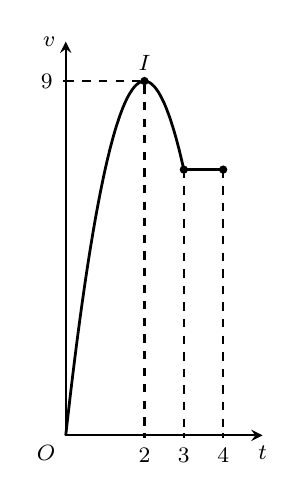
\begin{tikzpicture}[>=stealth,x=1.0cm,y=1.0cm,scale=0.5,thick]
			\draw[<->] (0,10) node[left]{\footnotesize $v$}--(0,0)--(5,0) node[below] {\footnotesize $t$};
			\foreach \x in {2,3,4}
			\draw[shift={(\x,0)},color=black] (0pt,2pt) -- (0pt,-2pt) node[below] {\footnotesize $\x$};
			\foreach \y in {9}
			\draw[shift={(0,\y)},color=black] (2pt,0pt) -- (-2pt,0pt) node[left] {\footnotesize $\y$};
			\draw (0,0) node[below left] {\footnotesize $O$};
			\draw[line width=1.0pt,color=black,smooth,domain=0:3] plot(\x,{-9*(\x)^2/4+9*\x});
			\draw[dashed] (0,9)--(2,9)--(2,0) (3,6.75)--(3,0) (4,6.75)--(4,0);
			\draw[line width=1.0pt,color=black] (3,6.75)--(4,6.75);
			\fill[black] (2,9) circle[radius=3pt] node[above]{\footnotesize $I$}(3,6.75) circle[radius=3pt] (4,6.75) circle[radius=3pt];
		\end{tikzpicture}
	}
	\loigiai{
		\begin{itemchoice}
			\itemch Dựa vào đồ thị của hàm vận tốc trên miền $t \in [0;4]$ thì $v_{\max}=9$ (km/h) khi $t=2$.
			\itemch Trên đoạn $t \in [0;3]$ thì đồ thị $v(t)$ là một parabol có đỉnh là $I(2;9)$ nên phương trình của nó có dạng $y=a(t-2)^2+9.$ Do parabol đi qua gốc tọa độ nên \[a(0-2)^2+9=0 \Leftrightarrow 4a+9=0 \Leftrightarrow a =-\dfrac{9}{4}.\]
			Vậy trên đoạn $[0;3]$ thì $v(t)=-\dfrac{9}{4}t^2+9t$.
			\itemch Với $t=3$ thì $v=\dfrac{27}{4}$. Trên đoạn $t \in [3;4]$ thì phần đồ thị là đường thẳng song song với trục hoành, suy ra $v(t)=\dfrac{27}{4}$ khi $t \in[3;4]$.
			\itemch Quãng đường mà vật di chuyển được trong $4$ giờ là
			$$s=\displaystyle\int\limits_0^3 \left (-\dfrac{9}{4}t^2+9t \right )\mathrm{\, d}t+\int\limits_3^4\dfrac{27}{4}\mathrm{\, d}t=27 \,\text{km}. $$
		\end{itemchoice}
	}
\end{ex}
\Closesolutionfile{ans}
\indapan{2}{ans/ans-2-OTC4-De1-DS}

\caukq
\Opensolutionfile{ans}[ans/ans-2-OTC4-De1-KQ]
\begin{ex}%[2D4H1-2]%Biên soạn:Phùng Hoàng Em %Phản biện:Nguyễn Đắc Kiên
	Cho $F(x)$ là một nguyên hàm của hàm số $f(x)=\dfrac{1}{x^2}$ thỏa mãn $F(2)=\dfrac{3}{2}$. Tính $F(1)$.
	\shortans{$1$}
	\loigiai{
		Ta có $F(x)=\displaystyle\int f(x)\mathrm{\,d}x= -\dfrac{1}{x}+C$. Vì $F(2)=\dfrac{3}{2}$ nên $-\dfrac{1}{2}+C=\dfrac{3}{2}\Leftrightarrow C=2$.\\
		Do đó, $F(x)=-\dfrac{1}{x}+2$.	Suy ra $F(1)=-\dfrac{1}{1}+2=1$.
	}
\end{ex}

\begin{ex}%[2D4V2-2]%Biên soạn:Phùng Hoàng Em %Phản biện:Nguyễn Đắc Kiên
	Cho hàm số $f(x)=\heva{&x^2+1 & \text{ nếu } x\geq 1\\&2x & \text{ nếu } x<1}$. Tính tích phân $\displaystyle\int\limits_0^2 f(x)\mathrm{\,d}x$ (\textit{làm tròn đến hai chữ số thập phân}).
	\shortans{$4{,}33$}
	\loigiai
	{Vì $\lim\limits_{x \to 1^+} f(x) = \lim\limits_{x \to 1^-} f(x)=f(1)=2$ nên hàm số $f(x)$ liên tục trên $\mathbb{R}$.\\
		Vì vậy $\displaystyle\int\limits_0^2 f(x)\mathrm{\,d}x = \displaystyle\int\limits_0^1 2x\mathrm{\,d}x + \displaystyle\int\limits_1^2 \left(x^2+1\right)\mathrm{\,d}x =1+ \dfrac{10}{3} = \dfrac{13}{3}\approx 4{,}33$.}
\end{ex}

\begin{ex}%[2D4H3-1]%Biên soạn:Phùng Hoàng Em %Phản biện:Nguyễn Đắc Kiên
	Tính diện tích $S$ của hình phẳng giới hạn bởi các đường $y=\mathrm{e}^x$, $y=2$, $x=0$, $x=1$ (\textit{làm tròn đến hai chữ số thập phân}).
	\shortans{$0{,}49$}
	\loigiai{
		Xét $\mathrm{e}^x=2 \Leftrightarrow x=\ln 2$.\\
		Diện tích hình phẳng giới hạn bởi các đường $y=\mathrm{e}^x$, $y=2$, $x=0$, $x=1$ là
		\begin{eqnarray*}
			S=\displaystyle\int_{0}^{1}\left|\mathrm{e}^x-2\right|\mathrm{\,d}x
			&=&\displaystyle\int_{0}^{\ln 2}\left|\mathrm{e}^x-2\right|\mathrm{\,d}x+\displaystyle\int_{\ln 2}^{1}\left|\mathrm{e}^x-2\right|\mathrm{\,d}x\\
			&=&-\displaystyle\int_{0}^{\ln 2}\left(\mathrm{e}^x-2\right)\mathrm{\,d}x+\displaystyle\int_{\ln 2}^{1}\left(\mathrm{e}^x-2\right)\mathrm{\,d}x\\
			&=& -\left.\left(\mathrm{e}^x-2x\right)\right|_0^{\ln 2}+\left.\left(\mathrm{e}^x-2x\right)\right|_{\ln 2}^{1}\\
			&=& -(2-2\ln 2-1)+(\mathrm{e}-2-2+2\ln 2)\\
			&=&4\ln 2+\mathrm{e}-5\approx 0{,}49.
		\end{eqnarray*}
	}
\end{ex}

\begin{ex}%[2D4V2-6]%Biên soạn:Phùng Hoàng Em %Phản biện:Nguyễn Đắc Kiên
	Giá trị trung bình của hàm số liên tục $f(x)$ trên đoạn $[a ; b]$ được định nghĩa là
	$$
	\dfrac{1}{b-a} \int_a^b f(x) \mathrm{\,d}x .
	$$
	Giả sử nhiệt độ ngoài trời ở một thành phố vào các thời điểm khác nhau trong ngày được mô phỏng bởi công thức $	h(t)=29+3 \sin \left[\dfrac{\pi}{12}(t-9)\right]$, với $h$ tính bằng độ $\mathrm{C}$ và $t$ là thời gian trong ngày tính bằng giờ.	Tìm nhiệt độ trung bình (đơn vị: độ) của ngày trong khoảng thời gian từ $6$ giờ sáng đến $12$ giờ trưa.
	\shortans{$29$}
	\loigiai{
	Nhiệt độ trung bình của ngày trong khoảng thời gian $6\le t \le 12$ được tính bởi công thức sau
\[\dfrac{1}{12-6} \int_6^{12} h(t) \mathrm{\,d}t=\dfrac{1}{6} \int_6^{12} \left( 29+3 \sin \left[\dfrac{\pi}{12}(t-9)\right]\right) \mathrm{\,d}t=29.\]
}
\end{ex}

\begin{ex}%[2D4C2-6]%Biên soạn:Phùng Hoàng Em %Phản biện:Nguyễn Đắc Kiên
Tại một nhà máy sản xuất một loại phân bón, gọi $P(x)$ là lợi nhuận (tính theo triệu đồng) thu được từ việc bán $x$ tấn sản phẩm trong một tuần. Khi đó, đạo hàm $P^{\prime}(x)$, gọi là lợi nhuận cận biên, cho biết tốc độ tăng lợi nhuận theo lượng sản phẩm bán được. Giả sử lợi nhuận cận biên (tính theo triệu đồng trên tấn) của nhà máy được ước lượng bởi công thức
$$
P^{\prime}(x)=16-0{,}02 x \text { với } 0 \leq x \leq 100.
$$
Tính lợi nhuận (triệu đồng) nhà máy thu được khi bán $90$ tấn sản phẩm trong tuần. Biết rằng nhà máy lỗ $25$ triệu đồng nếu không bán được lượng sản phẩm nào trong tuần.
	\shortans{$1334$}
\loigiai{
	Ta có $P(0)=-25$ (lỗ khi không bán được lượng sản phẩm nào trong tuần)
	$$
	\begin{aligned}
		P(90)-P(0) &=\displaystyle\int\limits_0^{90} P^{\prime}(x) \mathrm{\,d}x=\displaystyle\int\limits_0^{90}(16-0{,}02 x) \mathrm{\,d} x \\
		&=16 \displaystyle\int\limits_0^{90} \mathrm{\,d} x-0{,}02 \displaystyle\int\limits_0^{90} x \mathrm{\,d} x \\
		&=\left.16 x\right|_0 ^{90}-0{,}01 x^2\left.\right|_0 ^{90}=1359.
	\end{aligned}
	$$
	Suy ra $P(90)=P(0)+1359=-25+1359=1334$ (triệu đồng).\\
	Vậy lợi nhuận nhà máy thu được khi bán $90$ tấn sản phẩm trong tuần là $1334$ triệu đồng.
}
\end{ex}

\begin{ex}%[2D4C3-3]%Biên soạn:Phùng Hoàng Em %Phản biện:Nguyễn Đắc Kiên
	\immini[thm]
	{Gọi $(\mathscr{H})$ là hình phẳng giới hạn bởi đồ thị $(\mathscr{C})$ của hàm số $y=\sqrt{x}$, trục $Ox$ và đường thẳng $x=9$. Cho điểm $M$ thuộc đồ thị $(\mathscr{C})$ và điểm $A(9;0)$. Gọi $V_1$ là thể tích khối tròn xoay tạo thành khi hình phẳng $(\mathscr{H})$ quay quanh trục $Ox$, $V_2$ là thể tích khối tròn xoay tạo thành khi tam giác $OMA$ quay quanh trục $Ox$.}
	{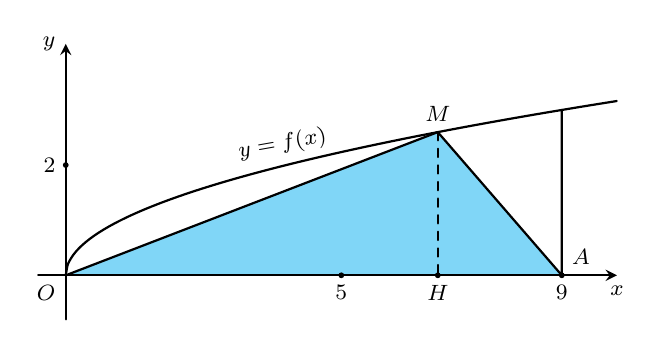
\begin{tikzpicture}[>=stealth,scale=0.7, line join=round, line cap=round,thick,font=\footnotesize]
			\def\xt{-0.5} \def\xp{10} \def\yt{4.2} \def\yd{-0.8}
			\fill[cyan!50!white](0,0)--(6.75,2.598)--(9,0)--cycle;
			\draw[->] (\xt,0)--(\xp,0) node [below]{$x$};
			\draw[->] (0,\yd)--(0,\yt) node [left]{$y$};
			\node at (0,0) [below left]{$O$};
			\node at (4,2) [above,rotate=10] {$y=f(x)$};
			\fill (0,2)node [left]{$2$} circle(1.5pt);
			\foreach \x in {5,9} \fill (\x,0)node[below]{$\x$} circle(1.5pt);
			\draw[smooth,samples=300,domain=0:10] plot(\x,{sqrt(\x)});
			\draw (0,0)--(6.75,2.598)--(9,0)--(9,3);
			\draw[dashed](6.75,2.598)--(6.75,0);
			\fill (6.75,2.598)node[above]{$M$} (9,3) (6.75,0)node[below]{$H$} circle(1.5pt);
			\node at (9,0)[above right]{$A$};
	\end{tikzpicture}}
	\vspace{0.3cm}
	\noindent
	Biết rằng $V_1=2V_2$. Tính diện tích $S$ phần hình phẳng giới hạn bởi đồ thị $(\mathscr{C})$ và đường thẳng $OM$ (\textit{làm tròn đến hàng phần trăm}).
	\shortans{$2{,}92$}
	\loigiai
	{Theo bài ra ta có $V_1=\pi\displaystyle\int\limits_{0}^{9}(\sqrt{x})^2\mathrm{\,d}x=\dfrac{81\pi}{2}$.\\
		Gọi $H$ là hình chiếu vuông góc của $M$ trên trục $Ox$.\\
		Đặt $OH=m$ (với $0<m<9$), khi đó $M(m;\sqrt{m})$, $MH=\sqrt{m}$, $AH=9-m$.\\
		Suy ra 
			\[V_2=\dfrac{1}{3}\pi\cdot MH^2\cdot OH + \dfrac{1}{3}\pi\cdot MH^2\cdot AH = \dfrac{1}{3}\pi\cdot MH^2\cdot OA = 3m\pi.\]
		Theo giả thiết $V_1=2V_2$ nên $\dfrac{81\pi}{2}=6m\pi \Leftrightarrow m=\dfrac{27}{4}$. Do đó $M\left(\dfrac{27}{4};\dfrac{3\sqrt{3}}{2}\right)$.\\
		Phương trình đường thẳng $OM$ là $y=\dfrac{2\sqrt{3}}{9}x$.\\
		Vậy diện tích hình phẳng giới hạn bởi đồ thị $(C)$ và đường thẳng $OM$ là
		$$S=\displaystyle\int\limits_{0}^{\tfrac{27}{4}} \left(\sqrt{x} - \dfrac{2\sqrt{3}}{9}x\right)\mathrm{\,d}x = \left(\dfrac{2}{3}x\sqrt{x}-\dfrac{\sqrt{3}}{9}x^2\right)\Bigg|_{0}^{\tfrac{27}{4}} = \dfrac{27\sqrt{3}}{16} \approx 2{,}92.$$
	}
\end{ex}

\Closesolutionfile{ans}
\indapan{6}{ans/ans-2-OTC4-De1-KQ}